% Native editable architecture with a checkpoint-bound test case and frozen results.
\begin{figure}[!t]
\centering
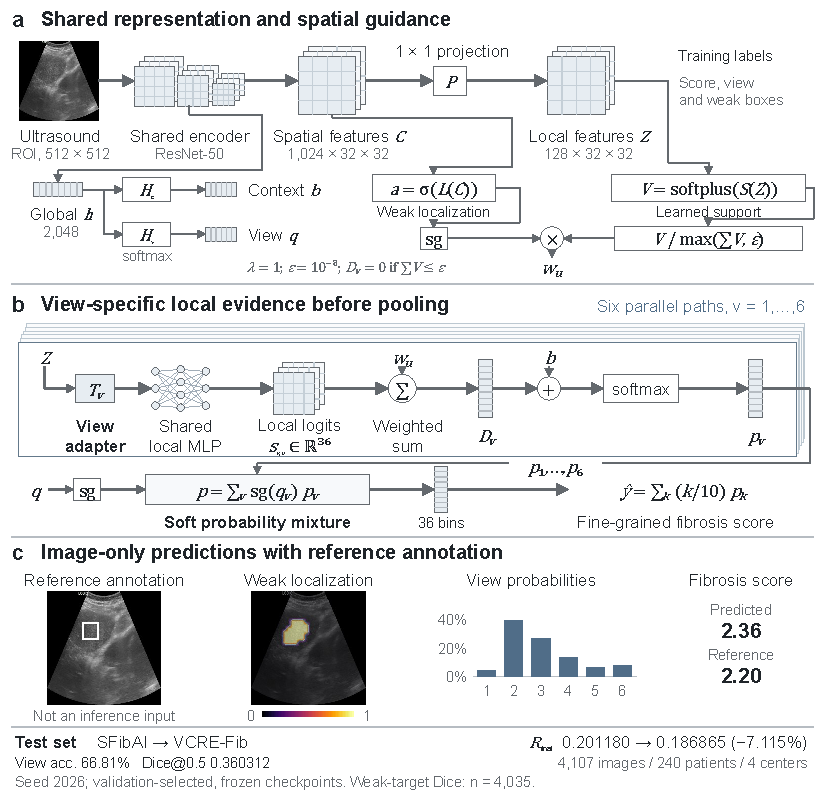
\includegraphics[width=\linewidth]{figures/assets/fig01_architecture.pdf}
\caption{\lang{\textbf{VCRE-Fib: view conditioning before spatial aggregation.} (a) A shared encoder supplies global context, view probabilities, weak localization and local features. (b) Six view-conditioned paths produce regional logit corrections, weighted by localization and learned support. Conditional distributions share context logits and are mixed by detached view probabilities. (c) One test case and test results from frozen, validation-selected checkpoints. Feature cells are schematic; $\sg$ denotes stop-gradient. Reference boxes are not inference inputs, and localization does not represent exhaustive segmentation.}{\textbf{VCRE-Fib：在空间聚合之前引入切面条件。}(a) 共享编码器提供全局上下文、切面概率、弱定位及局部特征。(b) 六条切面条件路径形成由定位与学习到的支持权重加权的区域 logit 修正。各条件分布共享上下文 logits，并依据截断梯度的切面概率融合。(c) 一个测试病例及使用经验证集选择并冻结的检查点得到的测试结果。特征格仅作示意，$\sg$ 表示停止梯度。参考框不参与推理，定位不表示完整病灶分割。}}\label{fig:architecture}
\end{figure}
